\documentclass{article}

\usepackage[utf8]{inputenc}
\usepackage{graphicx}
\usepackage[margin=1in]{geometry}
\usepackage[numbers,sort,]{natbib}
\usepackage{hyperref}
\usepackage[justification=centering]{caption}
\usepackage{subcaption}
\usepackage{amsmath}
\usepackage[subtle]{savetrees}

\hypersetup{
    colorlinks=true,
    linkcolor=black,
    urlcolor=blue,
    citecolor=black
}

\setlength{\bibsep}{0pt plus 0.3ex}

\title{Game Theory group coursework}
\author{Jagdev Bal, Ellie Fadipe, Jade Jones, Alex Room}
\date{}

\begin{document}

\maketitle

\section{Introduction}
Insider trading is the practice of purchasing or selling a publicly-traded company’s securities\footnote{i.e. assets which can be traded} while in possession of information that is not yet public (e.g. learning about a merger via dinner with the CEO). This practice may be illegal but is not uncommon in today's markets; insider traders enjoy better returns with less risk. This project sets out to investigate the relationship between strategies for both inside trading and its regulation. We test the effectiveness and change of a number of different strategies between inside traders and regulators under a co-evolutionary dynamic to see if there are superior strategies to avoid detection. 

This has been studied before in papers such as \citet{smales2017game}, who use Monte Carlo simulation. We instead use evolutionary dynamics to model these interactions.

\section{Methods}
Our stage game has two players, a trader $\mathcal{T}$ and a trading regulator $\mathcal{R}$, who are the row and column players respectively; the trader's actions as a 'regular' vs an 'insider' trade; the regulator's actions as 'no investigation' vs 'investigation'; and financial payoff matrices for both players as follows;
\begin{equation*}
\begin{split}
    \mathcal{T} = 
    \begin{pmatrix}
    1 & 1 \\
    6 & -10
    \end{pmatrix}
\end{split}
\quad\quad
\begin{split}
    \mathcal{R} = 
    \begin{pmatrix}
    1 & -1 \\
    -3 & 5
    \end{pmatrix}
\end{split}
\end{equation*}

i.e. a 'regular' trade has a small financial gain, but is immune to investigation - an insider trade, on the other hand, is much more lucrative but sustains heavy fines if caught. The regulator is punished on 'false positive' investigations and on failing to catch insider traders\footnote[2]{Statistical methods such as those in \citet{bris2005insider} can recognise that insider trading has occurred through passive stock market analysis, but not who is doing it.}, but are rewarded for catching fraud. 

\subsection{Information \& Evolution}
We note in our model that the two players do not have equal information. The trader always knows when they have been investigated, but the regulator can only be certain the trader has done inside trading if they have caught them doing it! Compare this to the Prisoner's Dilemma, where both players have full information.

We then create strategies for our game using the Axelrod library \citep{axelrodproject}. We have written code to implement asymmetric games into the library, and then used tournaments in those asymmetric games (matching each trader with each regulator) to simulate a 'paired Moran process'. 

This is a simplification of the graph-based Moran process \citep{shakarian2013novel}, which takes two populations - $P_1$ of row players, and $P_2$ of column players - and calculates the fitness of each member of each population against the \emph{other} population. With the Hawk-Dove game as an example, if $P_1 = \{\text{2 hawk, 1 dove}\}$ and $P_2 = \{\text{1 hawk, 2 dove}\}$, the fitness of the dove in $P_1$ is calculated based on its utilities against the 1 hawk and 2 doves in $P_2$. Birth and death for each population is then calculated from these fitnesses in the same way as the regular Moran process. This is done independently for each population (e.g. 1 birth and 1 death in $P_1$, \emph{and} 1 birth and 1 death in $P_2$)
\\

As opposed to the usual Moran process, this allows us to simulate situations where it may not be suitable for every player to interact with every other player; traders and regulators do not interact among themselves in the situation we are modelling, and asymmetric information means they do not necessarily share strategy spaces. This allows us to see how trading behaviour co-evolves with regulation behaviour over time, as separate yet dependent populations.

The outcome scores of each matchup in the tournament are an average of 500 matches of 500 repetitions each; the repetitions model consecutive trading days. We used 6 trading strategies, and 5 regulation strategies.

\section{Results}
\begin{figure}[!h]
  \begin{subfigure}[b]{0.4\textwidth}
    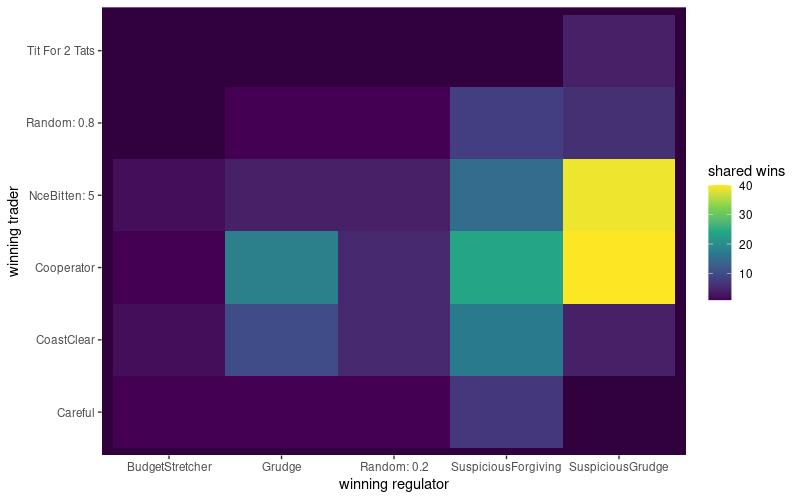
\includegraphics[width=\textwidth]{heatmap.png}
    \caption{A heatmap of co-winning trader-regulator pairs}
    \label{fig:f1}
  \end{subfigure}
  \hfill
  \begin{subfigure}[b]{0.4\textwidth}
    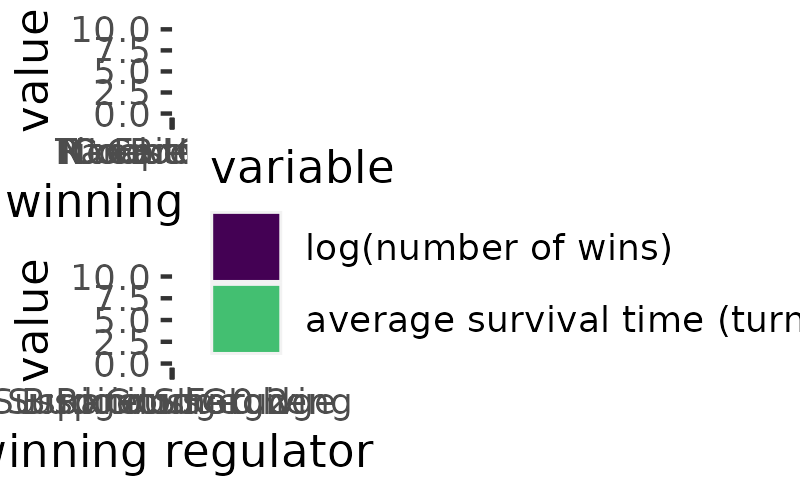
\includegraphics[width=\textwidth]{barplot.png}
    \caption{The number of wins and average survival time of each trader/regulator}
    \label{fig:f2}
  \end{subfigure}
\end{figure}

\section{Conclusion}
\bibliographystyle{unsrtnat}
\bibliography{bibliography}

\end{document}
